%%%%%%%%%%%%%%%%%%%%%%%%%%%%%%%%%%%%%%%%%%%%%%%%%%%%%%%%%%%%%%%%%%%%%%%%%%%%%
\chapter{Evaluierung}
\section{Vergleiche mit anderen Lösungen} 
Im Vergleich mit anderen Lösungen, die im Punkt 2.1 beschrieben werden, ergeben sich folgende Unterschiede und neue Aspekte: 
\begin{itemize}
\item Die Ergebnisse der Statischen Code Analyse werden über einen längeren Zeitraum gespeichert und nicht gelöscht. Dadurch kann auch die Historie der Fehler genauer analysiert werden. Die Fehler können nach Projekt und Datumsbereich gefiltert und angezeigt werden (siehe Abbildung \ref{fig:tableRec}).

\begin{figure}[tp]
  \centering
  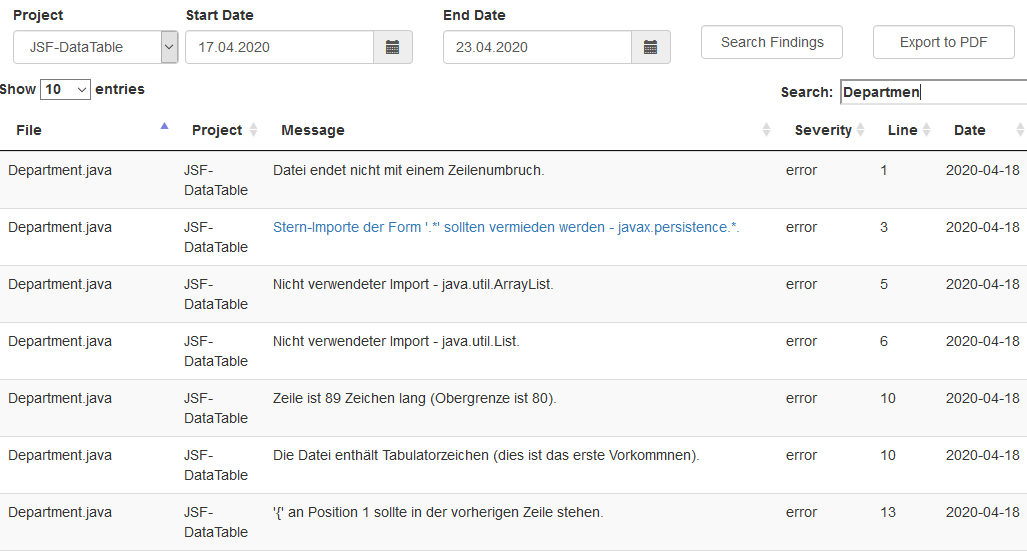
\includegraphics[height=8cm]{images/tableRec.PNG}
  % The short caption should be capitalised
  % The full caption should hold a full sentence. 
 \caption[Am häufigsten vorkommende Fehler in den ausgewählten Projekten.]{Am meisten vorkommende Fehler in den ausgewählten Projekten. (vgl. Fehler in den den Abbildungen \ref{fig:findingsInIDE} und \ref{fig:checkstyleHTMLReport})}
  \label{fig:tableRec}
\end{figure}

\item Durch das Plugin können eine Vielzahl an Tools unterstützt und eingebunden werden. Die einzige Voraussetzung hierbei ist das Angeben der XML-Results. Dadurch können die Benutzer die Applikation individuell gestalten, da nur die von ihnen gewünschten Fehler und Bugs analysiert werden können. Ein Einsatz beliebiger Tools für spezifische Probleme kann so unterstützt werden (siehe Punkt 2.3). Herkömmliche Lösungen wie Veracode oder SonarQube verwenden eine eingebaute und vorgegebene Code Analyse.
\item Aufgrund der Verwendung einer Web-Applikation ist das Springen, automatische Ausbessern und Navigieren zu den Fehlern, im Unterschied zu Entwicklungsumgebungen, nicht möglich. Die Fehler werden daher auch nicht direkt in der Entwicklungsumgebung markiert.
\item Im Frontend können Meldungen gezielt ignoriert werden (siehe Punkt 4.6.2.5). Dazu muss die bestimmte Meldung angegeben werden. In anderen Lösungen gibt es verschiedene Konzepte für diese Funktion, zum Beispiel das Hinzufügen von bestimmten Modulen mit denen man im Code Fehler ignorieren kann, mit Annotations oder mit Kommentaren. In anderen Lösungen können auch Code-Blöcke für die Analyse ausgenommen werden.
\item Mit dem Hinzufügen von Recommendations können Fehler vermieden werden (siehe Recommendation-Link in Abbildung \ref{fig:tableRec}). Das Ziel hierbei ist es auch, einen Lernprozess bei den Benutzerinnen und Benutzern zu ermöglichen. Herkömmliche Lösungen ermöglichen das automatische Ausbessern der Fehler oder geben zusätzliche  Informationen bei den Meldungen an.



\item Im Frontend können verschiedene Charts zur Unterstützung angezeigt werden. Auch andere Web-Lösungen wie SonarQube und Veracode ermöglichen das Anzeigen von Charts mit Informationen wie Anzahl der Fehlertypen oder Charts zur Komplexität der Fehler. In Entwicklungsumgebungen werden hingegen keine Charts angezeigt.
\end{itemize}
\section{Evaluierungen der Webapplikation mit Testpersonen} 
Die einzelnen Kriterien in den Beschreibungen der Evaluierung der Testpersonen werden im Punkt 1.2.2 genauer beschrieben. 

Die Testpersonen bewerten die einzelnen Punkte mit den Noten 1-5. Anmerkungen der Testpersonen werden zur Bewertung angegeben. Beim Kriterium \textit{Unterstützung} suchen die Testpersonen bestimmte Fehler  mithilfe der Applikation und bewerten die Fehlersuche im Vergleich zu herkömmlichen Lösungen bzw. zu einer freien Fehlersuche.
\subsubsection{Testpersonen}
\textbf{Testperson 1} \\
Erfahrung in der Softwareentwicklung: 5 Jahre Berufserfahrung; Erfahrung mit der Statischen Code Analyse: Bereits eingesetzt und verwendet \\
Bewertung der Kriterien:

Einfachheit: 2, Sub-Pages (Projekt, Charts, Suche, Übersicht) für eine bessere Unterteilung der Informationen \newline Übersicht: 2, Es sollte die Möglichkeit bestehen, einzelne Fehler genauer zu folgen, zum Beispiel wann genau der Fehler erstellt wurde. \newline  Unterstützung: 1, Fehler konnte in unter fünfzehn Sekunden gefunden werden, Besonders in Teams ist eine Git-Unterstützung notwendig um genauere Analysen und Informationen über die Entwickler zu bekommen.  \newline  Individualität: 1 \newline  Performance: 1 \newline  Verständnis: 2 \newline 

\textbf{Testperson 2} \\
Erfahrung in der Softwareentwicklung: 2 Jahre Berufserfahrung; Erfahrung mit der Statischen Code Analyse: Keine Erfahrungen\\
Bewertung der Kriterien:

Einfachheit: 3, Erstellung einer Dokumentation und Beispielen um die Verwendung des Programms (Plugins) genauer verstehen zu können. \newline  Übersicht: 1 \newline  Unterstützung: 2, Fehler konnte in unter zwanzig Sekunden gefunden werden; Hinzufügen einer Fehler-Historie, um Fehler genau verfolgen zu können und um Fragen beantworten zu können wie: Wann ist der Fehler das erste Mal aufgetreten? Wie lange war der Fehler im Projekt? \newline  Individualität: 1 \newline  Performance: 1 \newline  Verständnis: 1 \newline 

\textbf{Testperson 3} \\
Erfahrung in der Softwareentwicklung: 4 Jahre Berufserfahrung; Erfahrung mit der Statischen Code Analyse: Bereits eingesetzt und wird aktuell verwendet\\
Bewertung der Kriterien:

Einfachheit: 2, Mit einer Desktop-Applikation kann eine bessere Interaktion mit der Entwicklungsumgebung erfolgen \newline Übersicht: 1 \newline  Unterstützung: 1, Fehler konnte in unter fünfzehn Sekunden gefunden werden \newline Individualität: 2, Möglichkeit zur eigenen weiteren Einteilung der Fehler in Kategorien würde die Übersicht und die Individualität in der Webapplikation steigern.  \newline Performance: 1 \newline  Verständnis: 2, Angabe des eingesetzten Tools bei der Meldung\newline 

\textbf{Testperson 4} \\
Erfahrung in der Softwareentwicklung: 1 Jahr Berufserfahrung; Erfahrung mit der Statischen Code Analyse: Keine Erfahrungen\\
Bewertung der Kriterien:

Einfachheit: 3, Hinzufügen einer Dokumentation für das Einfügen der Plugins.  \newline Übersicht: 1 \newline  Unterstützung: 1, Fehler konnte in unter zwanzig Sekunden gefunden werden \newline Individualität: 2, Severity (Fehlerlevel) soll vom Benutzer auch selbst bestimmt werden können\newline Performance: 1 \newline  Verständnis: 2\newline 

\textbf{Testperson 5} \\
Erfahrung in der Softwareentwicklung: 2 Jahre Berufserfahrung; Erfahrung mit der Statischen Code Analyse: Bereits eingesetzt\\
Bewertung der Kriterien:

Einfachheit: 2, Hinzufügen einer Dokumentation für das Einfügen der Plugins.  \newline Übersicht: 2, Charts sollen in Pop-Ups angezeigt werden. Tabelle soll nach Packages gefiltert werden können \newline  Unterstützung: 1, Fehler konnte in unter fünfzehn Sekunden gefunden werden \newline Individualität: 1 \newline Performance: 1 \newline  Verständnis: 2, Bessere Erklärungen zu den Charts und zu den Feldern in der Tabelle (Schwere des Fehlers)\newline 

\textbf{Testperson 6} \\
Erfahrung in der Softwareentwicklung: 7 Jahre Berufserfahrung; Erfahrung mit der Statischen Code Analyse: Bereits eingesetzt und wird aktuell verwendet\\
Bewertung der Kriterien:

Einfachheit: 3, Hinzufügen einer Dokumentation für das Einfügen der Plugins; Erstellen von Container für die Docker-Unterstützung um die Applikation und die Datenbank schnell und einfach verwenden zu können; Erstellen einer Git-Integration und Möglichkeit zur Öffnung der Files in Github um die Fehler und Bugs direkt einsehen zu können \newline Übersicht: 2, Navigation zu den einzelnen Sections, Pfade der Klassen anzeigen, Zusätzlich zur Datum-Filterung auch Möglichkeit der Filterung nach Commit \newline  Unterstützung: 1, Fehler konnte in unter fünfzehn Sekunden gefunden werden \newline Individualität: 1, Erstellen eines Security-Tokens für die Sicherheit in der Applikation \newline Performance: 1 \newline  Verständnis: 1\newline 

\subsubsection{Interpretation der Evaluierungen}
\textbf{Einfachheit}
Durchschnittlicher Wert: 2,5\\
Die meisten Testpersonen, besonders Entwicklerinnen und Entwickler mit wenig Berufserfahrung, wiesen auf eine fehlende Dokumentation hin, insbesondere beim Einfügen und bei der Verwendung des Plugins. Eine Dokumentation und Beschreibung kann bei Tools wie Github hinzugefügt werden. Auch in der Webapplikation können Tooltips und Hilfe-Seiten für die Benutzung des Plugins hinzugefügt werden.

\textbf{Übersicht}
Durchschnittlicher Wert: 1,5\\
Bei diesem Kriterium erwähnten mehrere Testpersonen die Aufteilung der Applikation in mehrere Unter-Seiten. Ebenso eine genauere Betrachtung und Anzeige der Fehler und Charts(Historie und Pop-ups), könnte die Bewertung der Übersicht weiter steigern.

\textbf{Unterstützung}
Durchschnittlicher Wert: 1,2\\
Die hohe Bewertung bei der Unterstützung bestätigt die Möglichkeit zur Verbesserung des Codes der Entwicklerinnen und Entwickler. Einige Testpersonen erwähnten die Integration mit Tools für die Versionsverwaltung, um auch Team-Unterstützung integrieren zu können.

\textbf{Individualität}
Durchschnittlicher Wert: 1,4\\
Die Möglichkeit, verschiedene Tools für die Statische Code Analyse integrieren zu können, war ausschlaggebend für die Bewertung beim Kriterium der Individualität. Weitere Funktionalitäten wie die eigene Einteilung der Fehler in Kategorien und die Möglichkeit zur Erstellen eines Passworts für die Sicherung der Webapplikation würde die Individualität weiter steigern.

\textbf{Performance}
Durchschnittlicher Wert: 1,2\\
Der Wert der Performance zeigt, dass bei der Evaluierung keine größeren Performance-Probleme aufgetreten sind. Hierbei muss aber auch die Infrastruktur und die Menge der Daten bemerkt werden, die in der Praxis auch abweichen und so die Performance beeinflussen können.

\textbf{Verständnis}
Durchschnittlicher Wert: 1,7\\
Weitere Erklärungen zu den einzelnen Feldern in der Tabelle und zu den Charts könnten das Verständnis der Präsentationen der Daten verbessern.